\documentclass{article}
\usepackage[utf8]{inputenc}
\usepackage{amsmath,amssymb}
\usepackage{graphicx}
\usepackage[a4paper,margin=0.9cm]{geometry}
\usepackage{multicol}
\usepackage{sectsty}

\graphicspath{ {.} }

\DeclareMathOperator{\ima}{Im}
\newcommand\tab[1][0,5cm]{\hspace*{#1}}

\begin{document}
	\allsectionsfont{\small}
	\scriptsize
	
	\begin{multicols*}{3}
		\section{studio stabilità sistemi non lineari}
		\begin{enumerate}
			\item definisco gli equilibri (valori di \(x_1,x_2...,u\) per cui le derivate sono = 0 (usando le eq originali) )\\
			\item linearizzo il sistema rispetto ad un generico equilibrio (\(\overline{x_1},\overline{x_2},\overline{u}\)):\\
			definisco le variabili linearizzate \(\delta x' = A(\overline{x_1},\overline{x_2},\overline{u})\delta x\)... dove \(\delta x = x - \overline{x}\)\\ 
			poi faccio la derivata delle matrici A e B derivando rispetto a x (per A) e rispetto a u (per B)
			\item sostituisco in A i valori degli equilibri trovati in precedenza e se gli autoval sono negativi l'equilibrio è stabile
			
			
		\end{enumerate}
		\section{diagrammi di bode}
		\begin{itemize}
			\item Inizio del tracciamento: trovo g= numero di poli nell'origine - numero di zeri nell'origine
			\item pendenza modulo iniziale = -g
			\item fase iniziale = -90 * g e -180° se guadagno < 0
			\item poli con costante negativa es (1+s): -90° di fase e -1 di pendenza (con costante pos, aggiungi 90 di fase)
			\item zeri: contrario dei poli
			 
		\end{itemize}
		
		\textbf{risposte a scalino file funzioni di trasf pagina 25}\\
		Per risposta a scalino: trovare polo dominante (cost di tempo più grande in modulo), trovare Tass = 5/|1|, se c'è uno zero con cost di tempo < 0 c'è risposta inversa, se c'è con cost > 0 c'è sovraelongazione\\\\
		
		Per transitorio esaurito guardare guadagno e fase rispetto al guadagno e frequenza data dall'input\\\\
		\section{Criterio di bode e nyquist}
		\begin{itemize}
			\item Criterio di bode: si può applicare sse la fdt taglia i 0db e non ci sono poli con re>0 (1-s) allora il sistema retroazionato è AS sse guadagno > 0 e margie di fase a frequenza di taglio > 0
			\item criterio di nyquist: il sistema è AS sse il numero di giri antiorari attorno al numero -1 reale è definito (il diag non passa per -1) ed è uguale al numero di poli con re > 0 (1-s) \\
		\end{itemize}
	
		margine di guadagno = 1/modulo su frequenza di taglio\\
		
		
		\textbf{risposta a scalino di un sistema di controllo}\\
		\begin{itemize}
			\item se margine di fase > 75 --> come fdt di primo ordine basta trovare il tempo di ass
			\item altrimenti come fdt di secondo ordine, serve anche s% 
		\end{itemize}
		
		\textbf{Per creazione regolatore}
		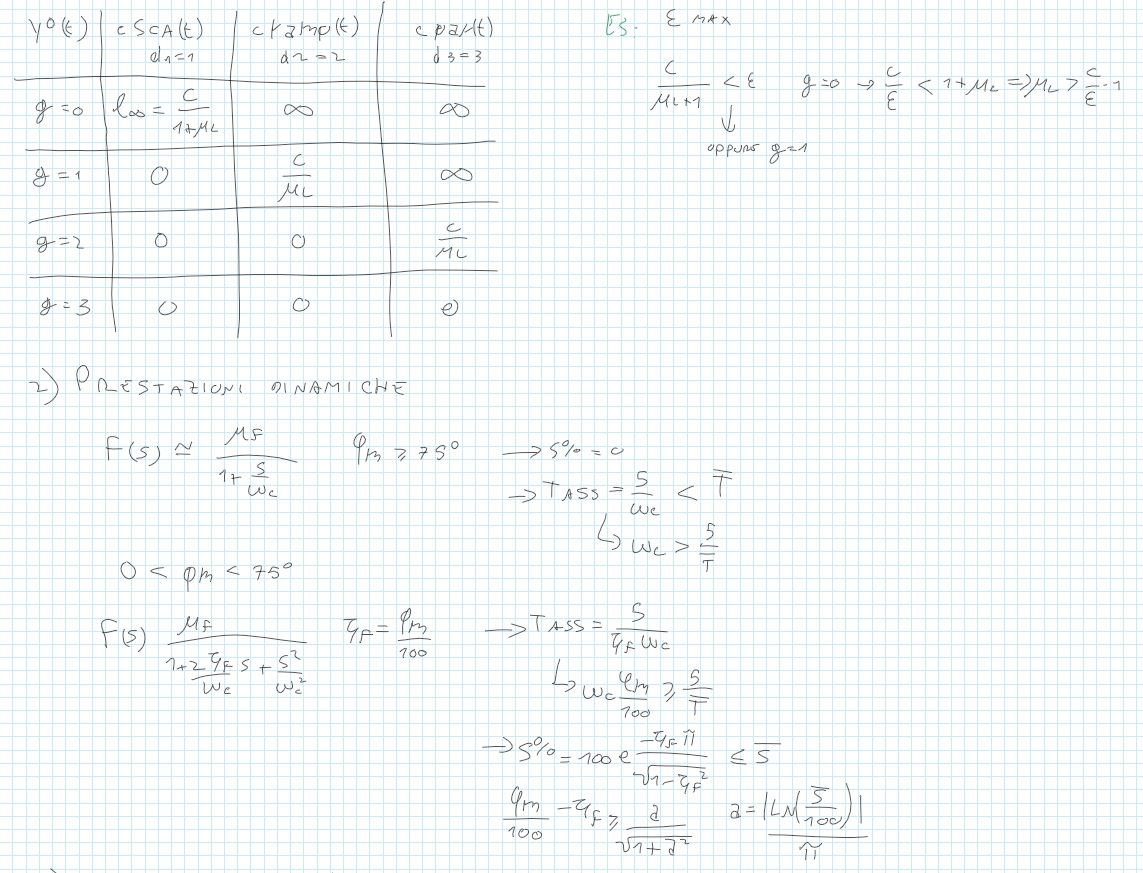
\includegraphics[scale=0.4]{regolatore}
		
		
		
		
		
		
		
		
		
		
		
		
		
		
		
		
		
		
		
		
	\end{multicols*}
\end{document}